% Geometry, font
\documentclass[12pt, letter]{article}
\usepackage[margin=0.8in]{geometry}
\usepackage[T1]{fontenc}
\usepackage{fourier}
\usepackage{titling}
\setlength{\droptitle}{-5em} 
\usepackage[parfill]{parskip}
\usepackage{graphicx}
\graphicspath{{imgs/}}
\usepackage{hyperref}

% Math stuff
\usepackage{amssymb}
\usepackage{bm}

% Code Highlighting
\usepackage{minted}
\usemintedstyle{solarizedlight}

\author{Zach Neveu}
\title{ Day 7 Notes }

\begin{document}
\maketitle

\section{Agenda}%
\label{sec:agenda}
\begin{itemize}
	\item Quiz
	\item Greedy Algorithms
	\item Intro to matching
	\item Announce next homework
	\item Announce next project
	\item Reading
\end{itemize}

\section{Greedy Algorithms}%
\label{sec:greedy_algorithms}
\begin{itemize}
	\item Classic Case: Minimum Spanning Tree
	\item Also useful for many other problems
	\item Single "greedy algorithm" really at the root of all of them
\end{itemize}

\subsection*{Head Partition (review from Day 6)}
\begin{itemize}
	\item Node-based solution - finds optimal solution
	\item Edge-based solultion - finds optimal solution, also very similar to MST
	\begin{itemize}
		\item Go edge-by-edge, add edge if it does not conflict
	\end{itemize}
\end{itemize}

\subsection*{Generic Greedy Algorithm}
\begin{minted}{Python}
def generalGreedy(g):
  sort(g.edges)
  soln = {}
  for edge in g.edges:
    if not conflicts(edge, soln)
    soln += edge
\end{minted}

\subsection*{Weighted Head Partition}
Given a weighted, directed graph, find an independent subset with maximum total weight.
\begin{itemize}
    \item Edge Strategy: Sort edges by decreasing weight. Starting with highest weight edge, add each edge if it does not conflict, else skip.
    \item Node Strategy: Go through nodes in any order and select the heaviest edge pointing to the given node
\end{itemize}

\subsection*{Partition}
\begin{itemize}
    \item Let $E$ be a finite set. $\pi$ is a partition of $E$ if it is a collection of disjoint subsets of $E$ such that the subsets collectively cover $E$.
    \item $E = \{e_1, \ldots, e_8\}$, $\pi = \big\{\{e_1\}, \{e_2, e_3\}, \{e_4, e_5\}, \{e_6, e_7, e_8\}\big\}$
    \item $\pi.weights = \big\{\{5\}, \{3, 4\}, \{7, 8\}, \{2, 6, 1\}\big\}$
    \item A subset of $E$ is \textbf{Independent} if no two elements come from the same component of $\pi$ 
    \item $\{e_1,e_4\}$ and $\{e_1,e_4,e_3\}$ are independent
    \item $\{e_1, e_2, e_3, e_4\}$ is not independent.
    \item Goal: given $E$ and $\pi$, find an independent subset of maximum weight.
    \item Strategy 1: from each component, select the largest element.
    \item Same as node strategy for head partition!

\end{itemize}

\subsection*{Maximum Weighted Matching}
\begin{itemize}
    \item Given a weighted graph, find a matching with the maximum total
    \item Simple greedy algorithm doesn't work!
    \item Simple algorithm will choose {{b,d}, {a,c}}, ignoring {{a,b}, {c,d}}
\end{itemize}

\begin{figure}[h]
    \centering
    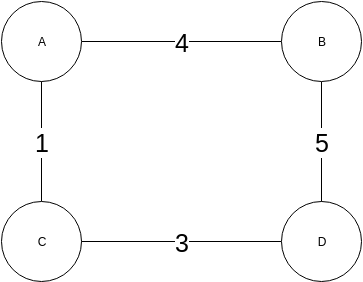
\includegraphics[width=0.5\textwidth]{weighted-matching}
    \caption{Weighted Matching Example}
    \label{fig:weighted-matching}
\end{figure}

\subsection*{Matching}
\begin{itemize}
    \item Given: a weighted graph and a matching M on the graph
    \item Edges in M are \textbf{matched edges} 
    \item Edges not in M are \textbf{free edges} 
    \item Nodes not adjacent to matched edges are \textbf{exposed} 
    \item Nodes that are adjacent to matched edges are \textbf{matched} 
    \item \textbf{Augmenting Path}: a simple path in the graph beginning and ending at exposed nodes, and alternating between crossing matched and free edges.
    \item Augmenting Path example in \ref{fig:matching}: $(v_1,v_4,v_5,v_6,v_8,v_7,v_{10},v_9)$
    \item Augmenting Path length always odd because start and end must be on exposed nodes.
    \item Finding longest augmenting path same as finding largest matching
    \item Given an augmenting path, swapping edges membership in M along the path creates a valid matching with length one longer.
\end{itemize}

\begin{figure}[h]
    \centering
    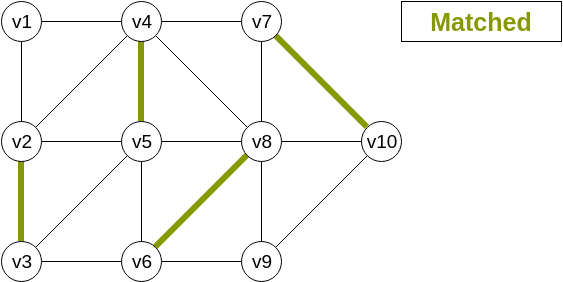
\includegraphics[width=0.8\textwidth]{matching}
    \caption{Matching Example}
    \label{fig:matching}
\end{figure}
\end{document}
